\documentclass[a4paper,10pt,titlepage]{report}

\usepackage[utf8]{inputenc}
\usepackage[T1]{fontenc}
\usepackage[english]{babel}
\usepackage{amssymb}
\usepackage{amsmath}
\usepackage{amsthm}
\usepackage{graphicx}
\usepackage{fancyhdr}
\usepackage{lastpage}
\usepackage{listings}
\usepackage{algorithm}
\usepackage{algpseudocode}
\usepackage[document]{ragged2e}
\usepackage[margin=1in]{geometry}
\usepackage{enumitem}
\usepackage{color}
\usepackage{datenumber}
\usepackage{venndiagram}
\usepackage{chngcntr}
\usepackage{mathtools}
\usepackage{booktabs}
\setcounter{tocdepth}{4}
\DeclarePairedDelimiter{\ceil}{\lceil}{\rceil}

%lstlisting ting:
\definecolor{dkgreen}{rgb}{0,0.45,0}
\definecolor{gray}{rgb}{0.5,0.5,0.5}
\definecolor{mauve}{rgb}{0.30,0,0.30}
\lstset{frame=tb,
  language=C,
  aboveskip=3mm,
  belowskip=3mm,
  showstringspaces=false,
  columns=flexible,
  basicstyle={\small\ttfamily},
  numbers=left,
  numberstyle=\footnotesize,
  keywordstyle=\color{dkgreen}\bfseries,
  commentstyle=\color{dkgreen},
  stringstyle=\color{mauve},
  frame=single,
  breaklines=true,
  breakatwhitespace=false
  tabsize=1
}
\lstset{literate=%
{æ}{{\ae}}1
{å}{{\aa}}1
{ø}{{\o}}1
{Æ}{{\AE}}1
{Å}{{\AA}}1
{Ø}{{\O}}1
}
\lstset{extendedchars=\true}
\lstset{inputencoding=ansinew}
\renewcommand{\lstlistingname}{Code} 

\setdatetoday
\addtocounter{datenumber}{0} %date for dilierry standard is today
\setdatebynumber{\thedatenumber}
\date{}


\setcounter{section}{-1}
\setcounter{tocdepth}{3}
\setcounter{secnumdepth}{2}


\pagestyle{fancy}
\fancyhf{}
\title{CC - Assignment 3}

\newcommand{\Z}{\mathbb{Z}}
\lhead{Compiler (DM546)}
\rhead{Mjerv15, Trpet15  \& Mojae15}
\rfoot{Page  \thepage \, of \pageref{LastPage}}
\counterwithin*{equation}{section}

\begin{document}
\newpage
{%
\centering
    \huge
    \bfseries
    \vspace{5mm}
CC, Spring 2018\\
Exam project, part 3\\
\vspace{5mm}
\begin{tabular}{|l|l|}
\hline
Group & 1 \\ \hline
\end{tabular}
\\
\vspace{10mm}
\begin{tabular}{@{}ll@{}}
\toprule
\multicolumn{1}{|l|}{Name}      & \multicolumn{1}{l|}{Mark Wolff Jervelund } \\ \midrule
\multicolumn{1}{|l|}{Birthday}  & \multicolumn{1}{l|}{280795} \\ \midrule
\multicolumn{1}{|l|}{Login}     & \multicolumn{1}{l|}{mjerv15@student.sdu.dk} \\ \midrule
\multicolumn{1}{|l|}{Signature} & \multicolumn{1}{l|}{\includegraphics[scale=0.3]{mark_sign}} \\ \midrule
                                &                       \\ \midrule
\multicolumn{1}{|l|}{Name}      &  \multicolumn{1}{l|}{Troels Blicher Petersen} \\ \midrule
\multicolumn{1}{|l|}{Birthday}      &   \multicolumn{1}{l|}{230896} \\ \midrule
\multicolumn{1}{|l|}{Login}      &  \multicolumn{1}{l|}{trpet15@student.sdu.dk} \\ \midrule
\multicolumn{1}{|l|}{Signature}      & \multicolumn{1}{l|}{\includegraphics[scale=0.08]{troels_sign} } \\ \midrule
                                &                       \\ \midrule
\multicolumn{1}{|l|}{Name}     &  \multicolumn{1}{l|}{Morten Kristian Jæger} \\ \midrule
\multicolumn{1}{|l|}{Birthday}      &  \multicolumn{1}{l|}{030895} \\ \midrule
\multicolumn{1}{|l|}{Login}     &   \multicolumn{1}{l|}{mojae15@student.sdu.dk} \\ \midrule
\multicolumn{1}{|l|}{Signature}    &  \multicolumn{1}{l|}{\includegraphics[scale=0.3]{morten_sign}} \\ \midrule
\end{tabular}
\\
\vspace{10mm}
This report contains a total of \underline{ \pageref{LastPage} } pages.
}

\begin{titlepage}
\centering
    \vspace*{9\baselineskip}
    \huge
    \bfseries
    3. Assignment \\
    \normalfont 
    Mark Jervelund, Troels Blicher Petersen \& Morten Jæger  \\
    (Mjerv15, Trpet15, Mojae15) \\
	\huge    
    Compiler (DM546)  \\[4\baselineskip]
    \normalfont
	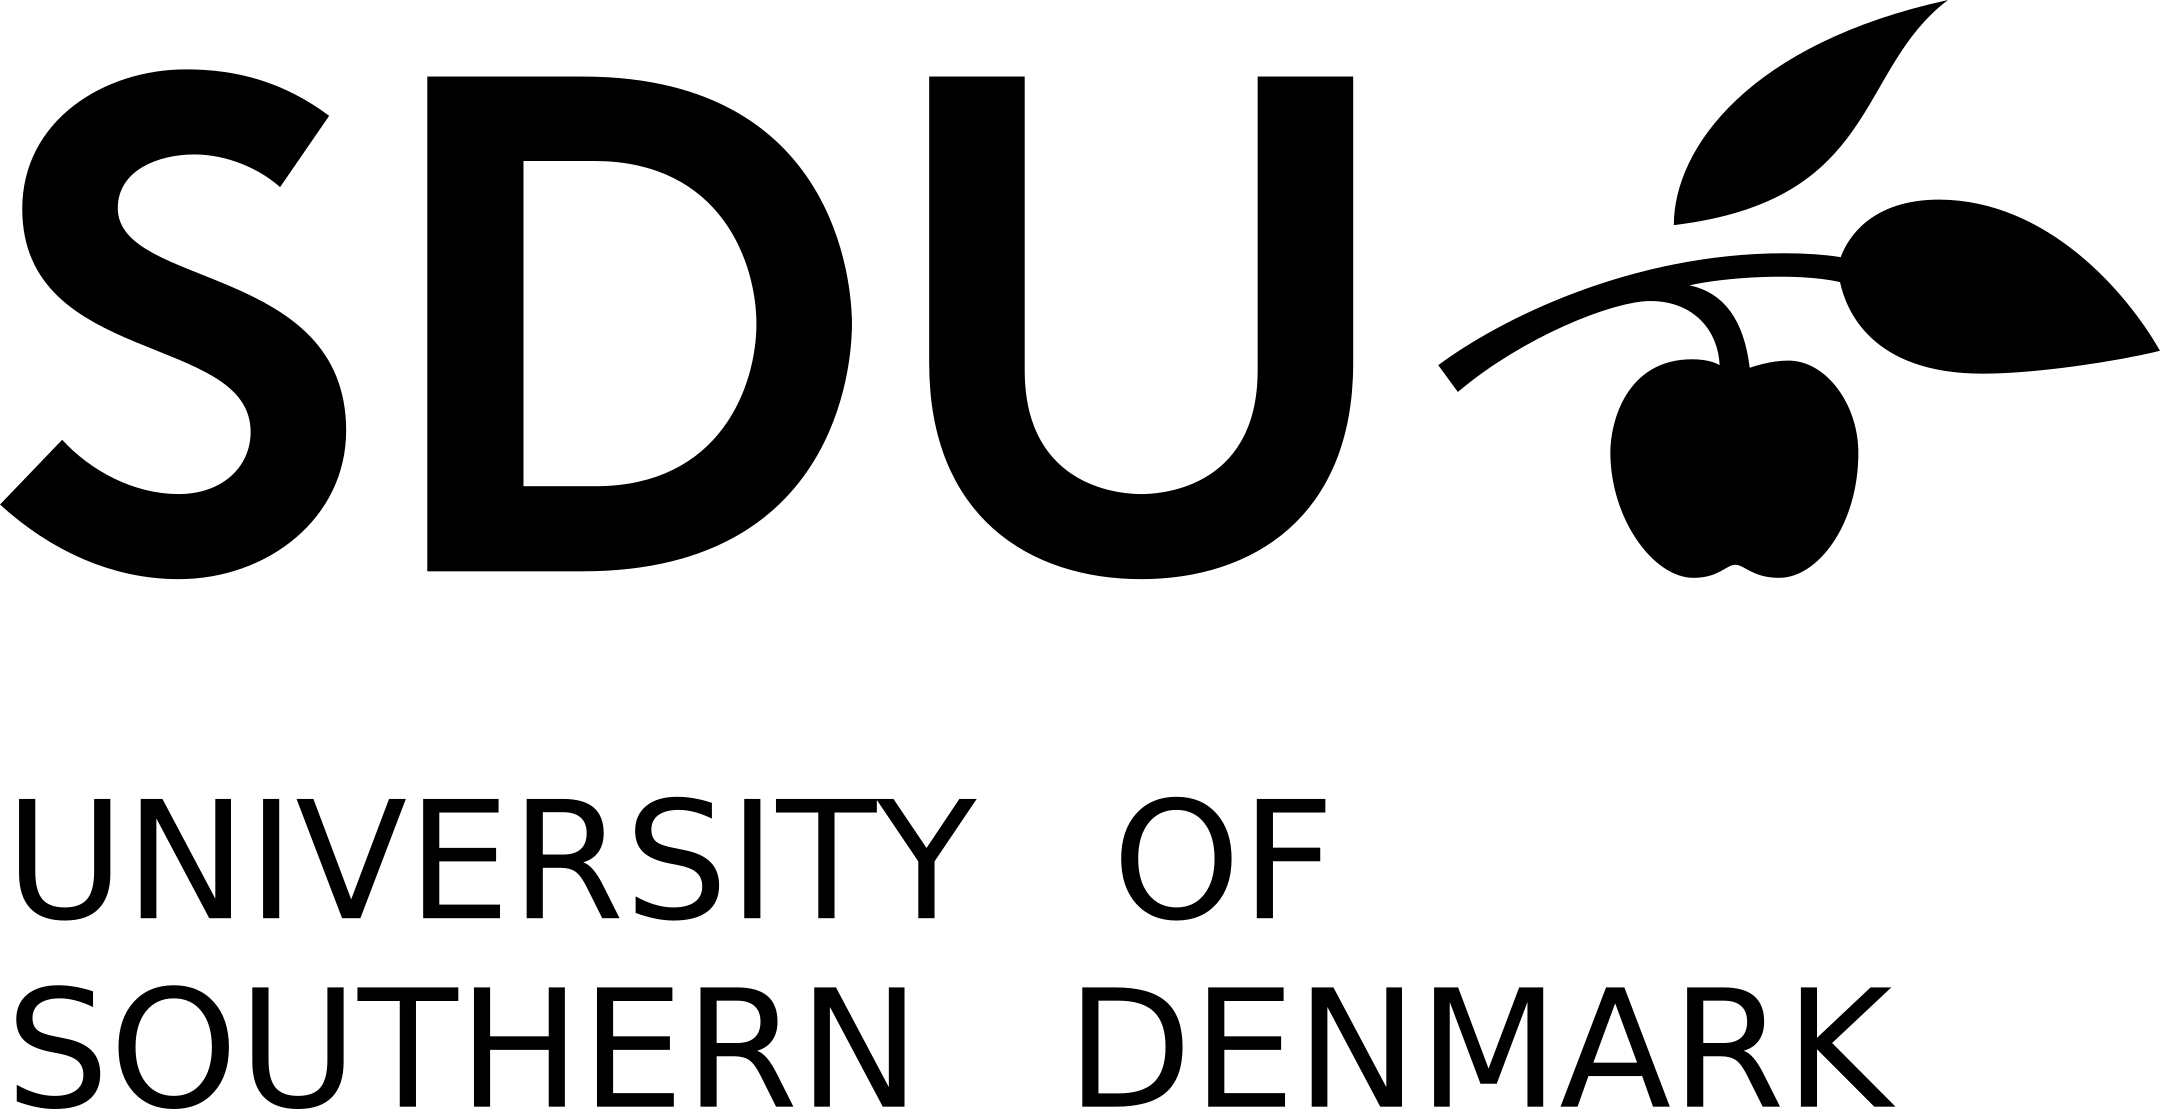
\includegraphics[scale=1]{SDU_logo}
    \vfill\ 
    \vspace{5mm}
    IMADA \\

    \textbf{\datedate} \\[2\baselineskip]
\end{titlepage}

\renewcommand{\thepage}{\roman{page}}% 
\tableofcontents
\newpage
\setcounter{page}{1}
\renewcommand{\thepage}{\arabic{page}}


\newpage
\section{notes}
Book \\
https://github.com/yihui-he/Modern-Compiler-Implementation-in-C/blob/master/Modern%20Compiler%20Implementation%20in%20C.pdf

\subsection{02/02-18}
Tools:\\
flex, bison,\\
Intel Pentium \\
0\\

\subsubsection{Phases of a modern compiler}
\textbf{Scan(Leksikalsk analyse):}\\
build a abstract syntax tree, and check if the programs contains any illegal symbols or identifiers.\\
The allowed items are \{, \}, (, ),=,+ -, <=, =>, return, "numbers", ""Strings"", indentifiers. comments are removed, as they are only meant for the code writer. \\
\vspace{6px}
\textbf{Parse:}\\
\vspace{6px}
\textbf{Weed:}\\
\vspace{6px}
\textbf{Symbol:}\\
Opsaml information om variabler\\
\vspace{6px}
\textbf{Type:}\\
Er sproget typekorrekt? eg. 42 + "ko"? Angiv et sæt regler, så tingene kommer i orden efter design-valg.\\
\vspace{6px}
\textbf{Resource:}\\
Har man resourcer tilgængelige?\\
\vspace{6px}
\textbf{Code:}\\
Generer kode \\
\vspace{6px}
\textbf{Optimize:}\\
Optimer genererede kode\\
\vspace{6px}
\textbf{Emit:}\\

\subsubsection{Regulære udtryk - Regular Expressions}
\begin{table}[H]
\caption{Regular expression operations.}
\begin{tabular}{l|l|l}
Symbol        & a         & \{a\}                           \\
\hline
Altering      & $M|N$       & $L(M) \cup L(N)$                  \\
\hline
Concatenating &$ M \cdot N$ &$ \{xy | x \in L(M), y \in L(N) $  \\
\hline
Epsilon      &$ \epsilon $   &$ \{\epsilon\} or \{""\} $        \\
\hline
Repetition(Kleene star)      & M*    &$ \{\epsilon \} \cup L(M \cdot M) \cup L(M\cdot M\cdot M) \cup ....$         \\
\end{tabular}
\end{table}

\subsubsection{Regulære udtryk - Regular Expressions - Forkortelser}
\begin{table}[H]
\caption{Forkortelser for Regular Expressions}
\begin{tabular}{l|l}
[abcd]        & (a|b|c|d)                                    \\
\hline
[d-g]     & ([defg]       \\
\hline
[d-gB-Dxq-s] & [defgBCDxqrs]  \\
\hline
M?      & $(M| \epsilon)$        \\
\hline
$M^+$     & $M\cdot M^*$         \\
\hline
. & [abc...012...+-/..] Uden Newline \\
\hline

\end{tabular}
\end{table}

\subsubsection{Flex - Fast Lexical Analysis}
\textbf{Flex format}\\
\%\{ \\
\hspace{6px} c-definitioner\\
\}\% \\
\vspace{6px}
\textbf{Flex-def:}\\
Definitioner og udtryk\\
Example: digits [0-9]\\
\vspace{6px}
yytext\\
yyleng\\
yyval\\
\vspace{6px}
\textbf{Flex regler}\\
1. Længste match\\
2. Regel prioritet\\
\vspace{6px}
\textbf{How to run Flex:}\\
\textsf{> flex FILENAME.l -> lex.yy.c\\
> gcc lex.yy.c -> a.out \\
> ./a.out < INPUTFILE \\
> echo INPUTFILE | a.out
}
\subsection{06/02-18}

\subsubsection{Scanners and Parsers}



























\newpage

\section{Introduction}

\subsection{Clarifications}

\subsection{Limitations}

\subsection{Extensions}

\subsection{Implementation Status}

\section{Parsing and Abstract Syntax Trees}

\subsection{The Grammar}

\subsection{Use of the {\tt flex} Tool}

\subsection{Use of the {\tt bison} Tool}

\subsection{Abstract Syntax Trees}

\subsection{Syntactic Sugar}

\subsection{Weeding}

\subsection{Test}

%%We should write some shit here.
\section{The Symbol Table}
The symbol table works like a standard extendible hash table, It's function is to store our symbols in
\subsection{Scope Rules}

\subsection{Symbol Data}

\subsection{The Algorithm}
\textcolor{red}{Hashing Algorithm ?}

\subsection{Test}
Write test from the other reports. give a example but keep it mainly text based.

\section{Type Checking}

\subsection{Types}

\subsection{Type Rules}

\subsection{The Algorithm}

\subsection{Test}

\section{Resource Computations}

\subsection{Resources}

\subsection{The Algorithm}

\subsection{Test}

\section{Code Generation}

\subsection{Strategy}

\subsection{Code Templates}

\subsection{The Algorithm}

\subsection{Test}

\section{Phases before Emit}

\subsection{Analyses}

\subsection{Algorithms}

\subsection{Test}

\section{Emit}

\subsection{Example Code}

\subsection{Test}

\section{Conclusion}

\newpage

\appendix

\section{Source Code}


\end{document}
